\chapter{Suitability of tracks as fake proxies}
\label{app:MOSSFlepton,track}

\subsubsection{Low-quality leptons showing up as tracks}
Note: This section currently has 8 TeV information and has not been updated

Out of curiosity, we look at the invariant mass of an opposite-sign muon+track pair. If the tracks are uncorrelated with the muons, we expect a broad peak at the average invariant mass. If they are correlated, they will be related to their source, for example a \Z decay. In fact, we see both (Figure~\ref{fig:app:MOSSFlepton,track}).

\begin{figure}
\begin{center}
	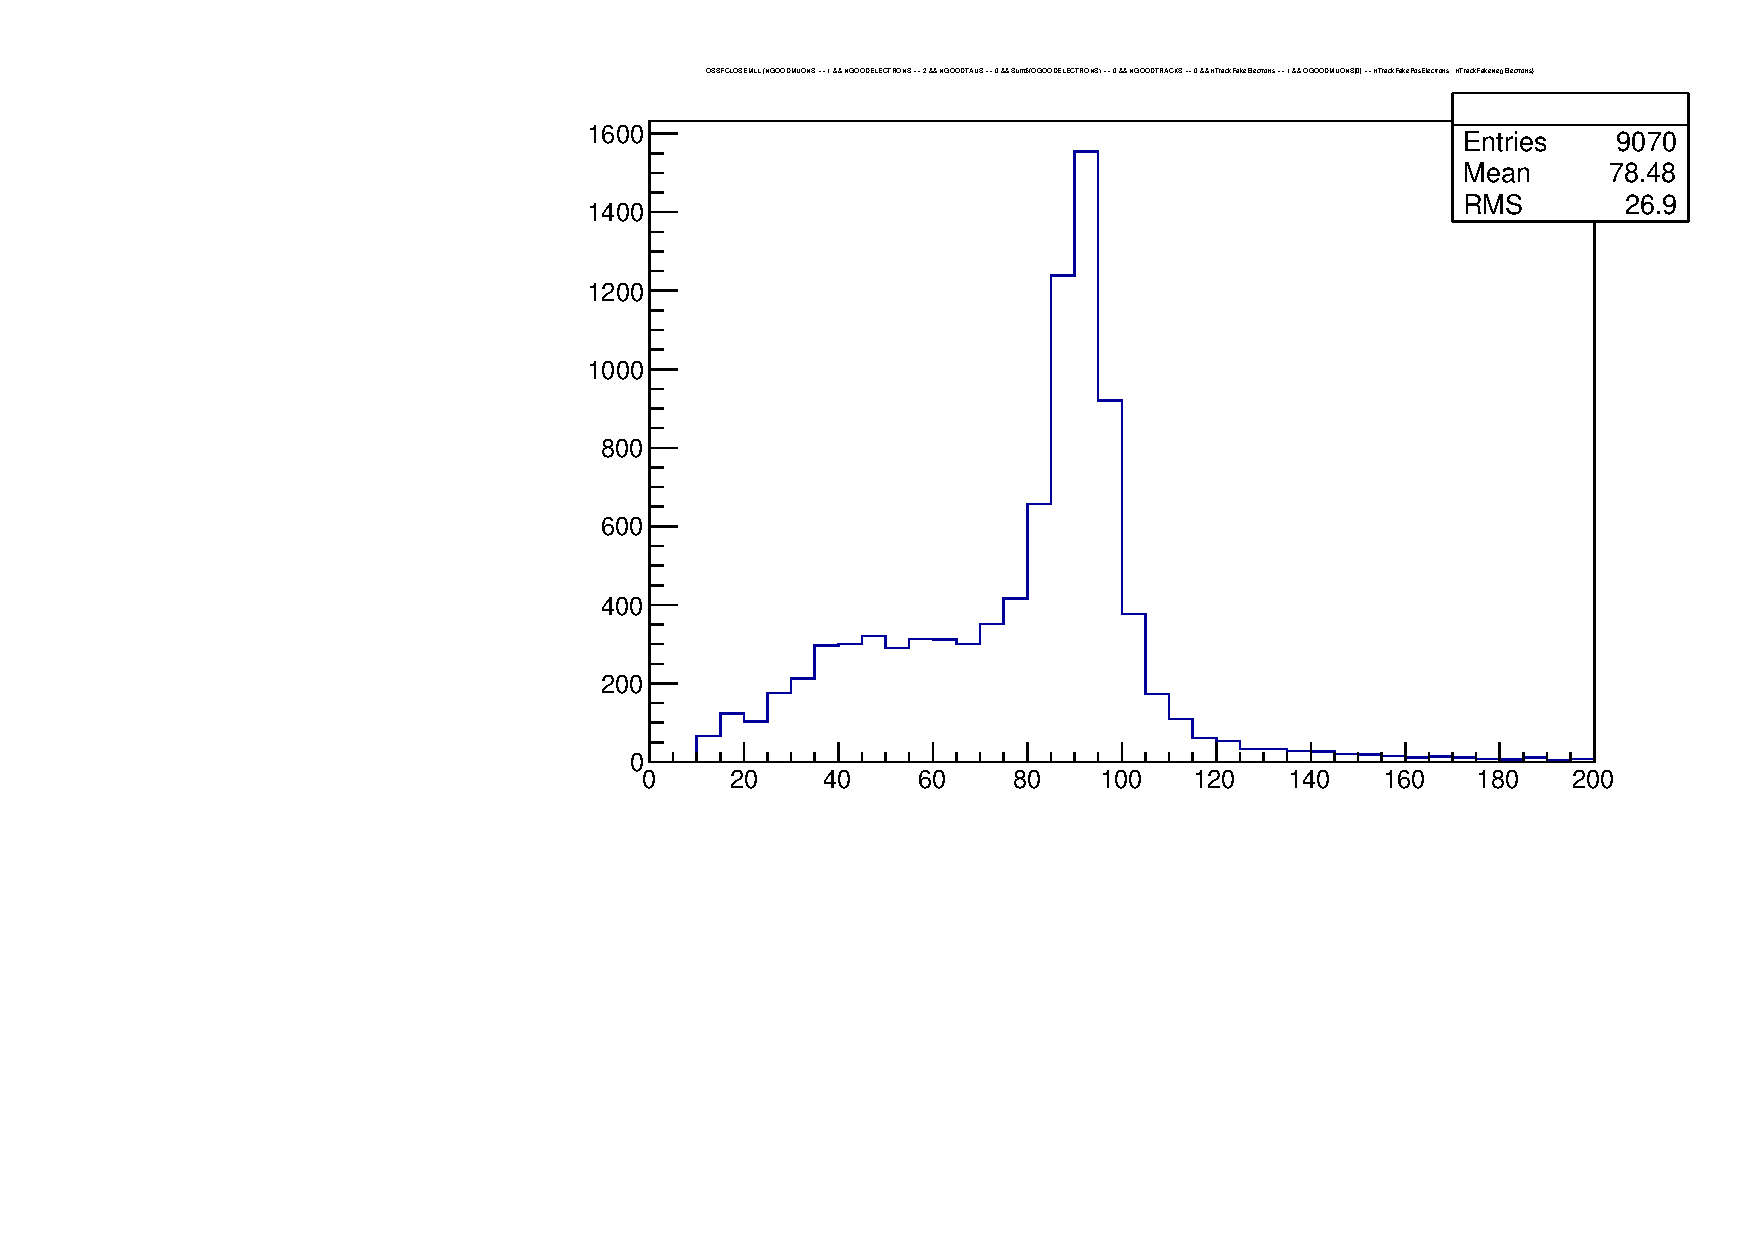
\includegraphics[width=.5\textwidth]{Appendix/study_OSSFCLOSEMLL_electron,track_1fake}%
	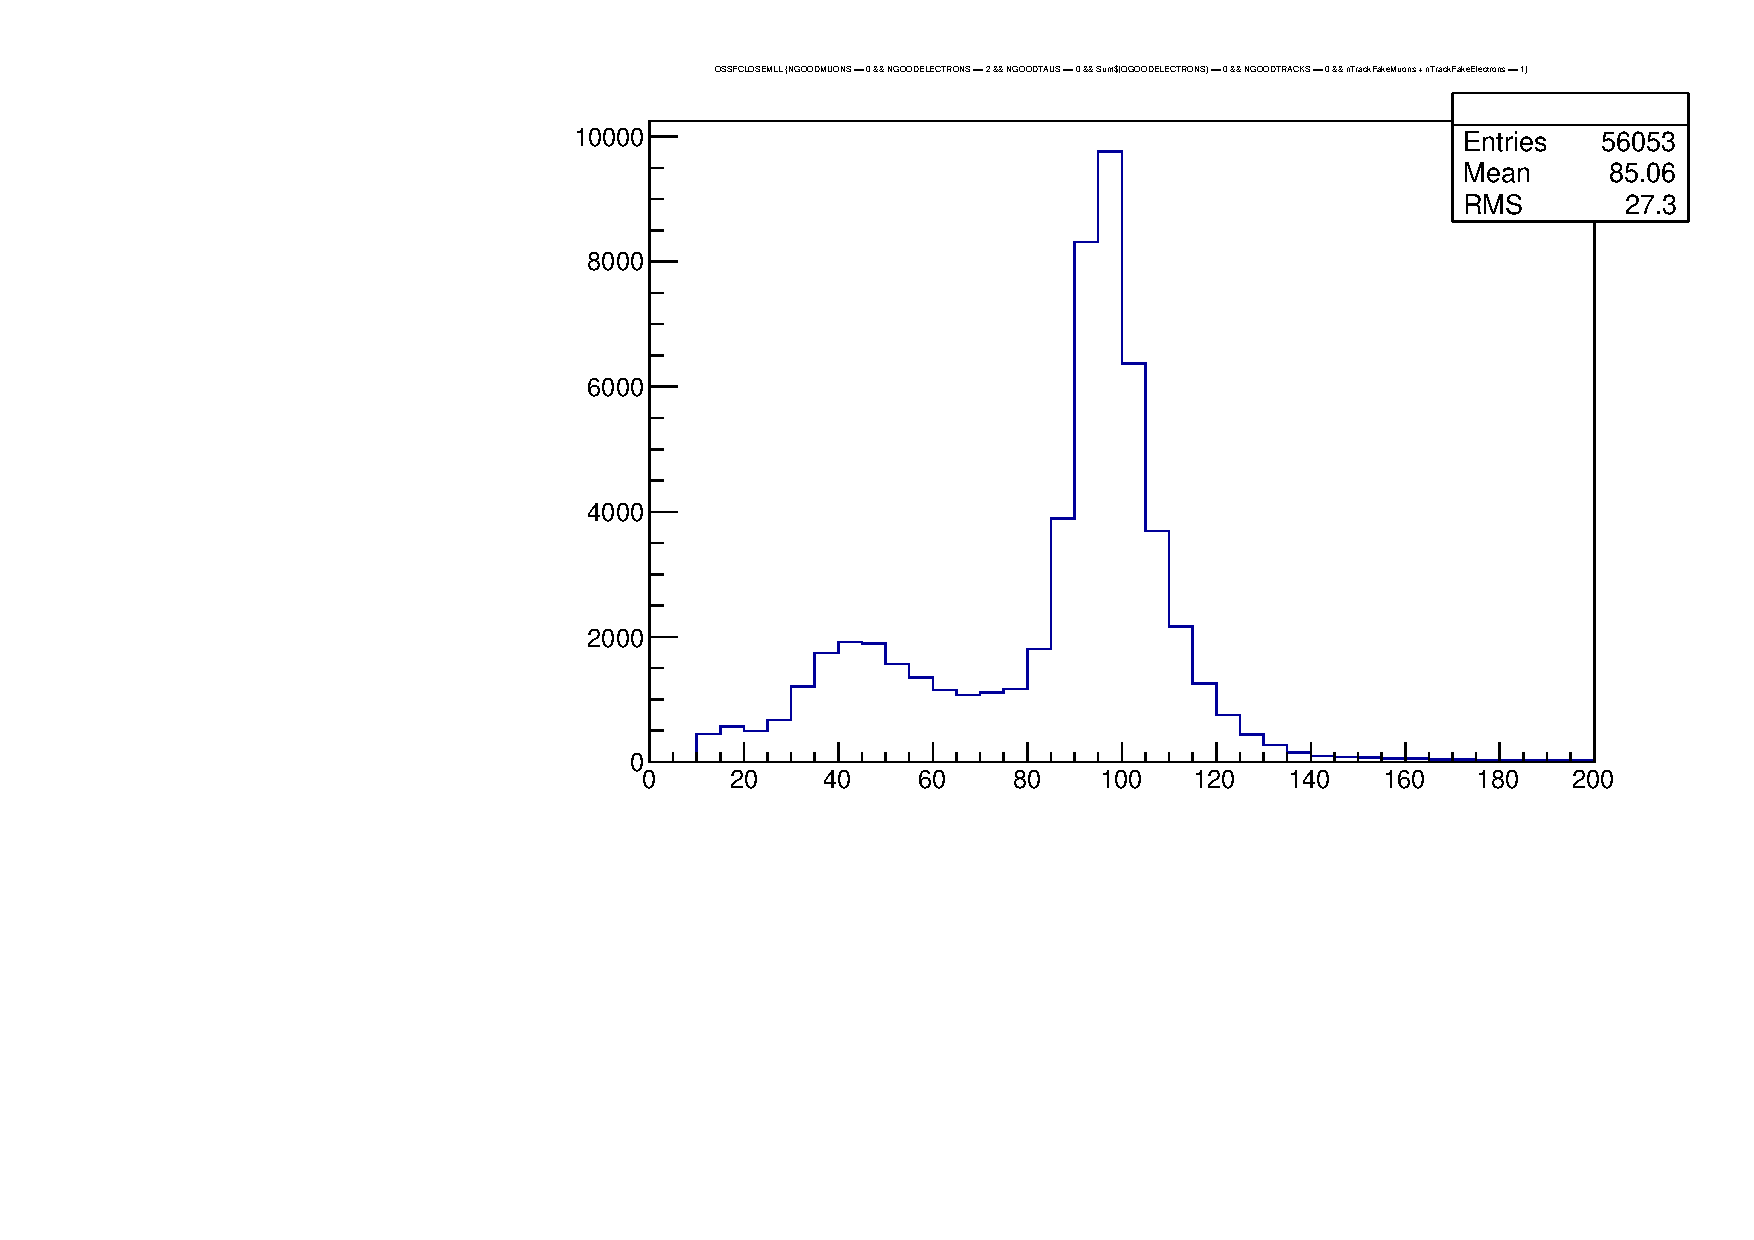
\includegraphics[width=.5\textwidth]{Appendix/study_OSSFCLOSEMLL_electron,track_dileptons-1fake}\\
	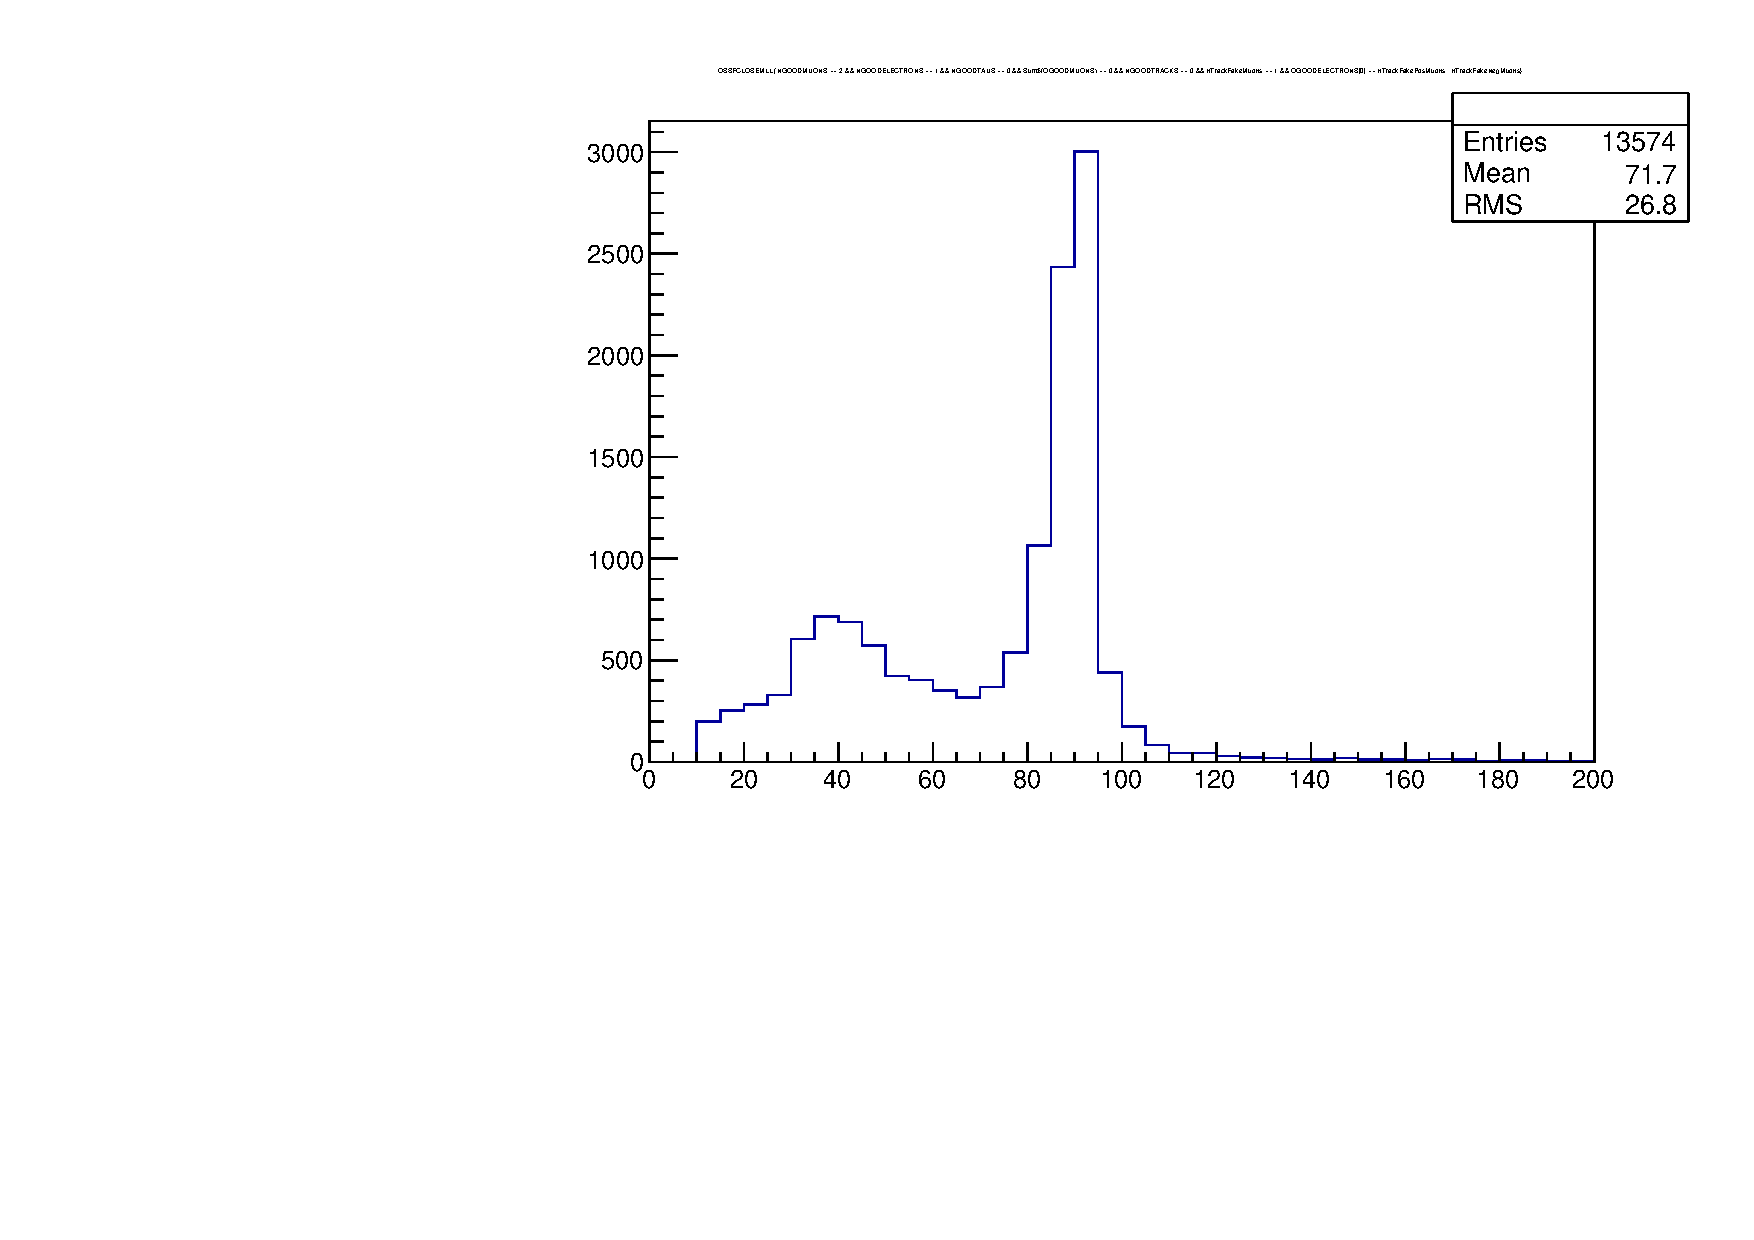
\includegraphics[width=.5\textwidth]{Appendix/study_OSSFCLOSEMLL_muon,track_1fake}%
	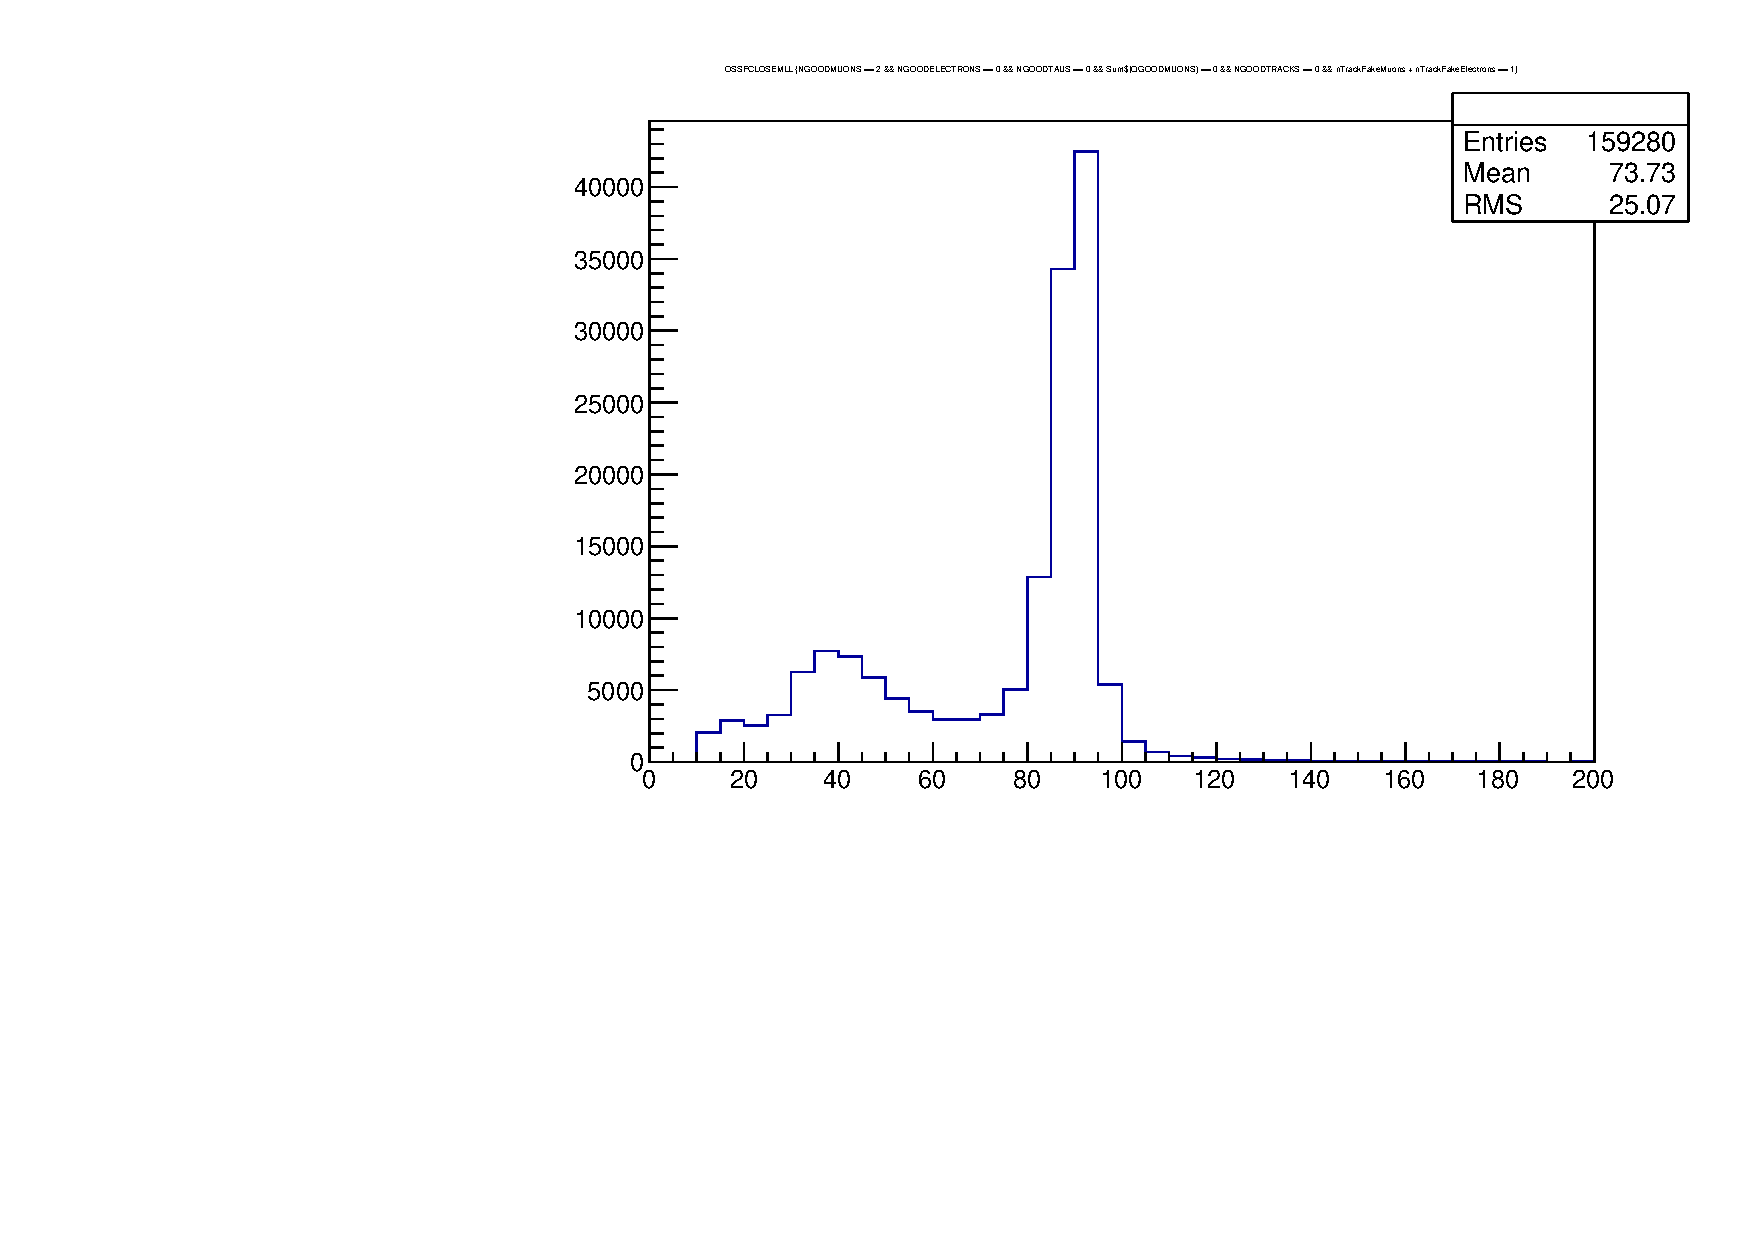
\includegraphics[width=.5\textwidth]{Appendix/study_OSSFCLOSEMLL_muon,track_dileptons-1fake}
	\caption{Top: $m_{et}$ distribution; bottom: $m_{\mu t}$ distribution. Left: no other leptons present, right: additional lepton present. If a third lepton is present, its flavor is opposite the flavor of the first lepton, and its charge is the same as the track's (rejecting third leptons from \Z).\\
	\textbf{Note:} This is from the dilepton-triggered dataset, i.e. the tracks used here probably were good enough leptons to trigger.
	\label{fig:app:MOSSFlepton,track}}
\end{center}
\end{figure}

This suggests that tracks are not only from jets, but also from low quality leptons. So, tracks do model fake leptons from jets, and at the same time also model leptons that were vetoed by quality cuts. However, the general shape of the track background is still expected to be in agreement with the shape of the signal regions. \fixme{Does that make sense? Also, understand the left--right difference in Figure~\ref{fig:app:MOSSFlepton,track}?}
